% !TeX root = ../../../main.tex
\subsection{Method}

We now introduce \ChTwoSmallCaps{Temporal-SCL}, our temporal adaptation of SCL.
It consists of three networks: an encoder $f$, a predictor $g$, and a temporal network $h$. 
We give a high-level overview of these networks in Section~\ref{ch02:sec:overview-networks} and how they are trained and used for prediction in Section~\ref{ch02:sec:training}.
We propose a method for visualizing embedding vectors in Section~\ref{ch02:sec:visualizing}.



\subsubsection{Overview of \ChTwoSmallCaps{Temporal-SCL}'s Networks}
\label{ch02:sec:overview-networks}

 

\noindent
\textbf{Encoder network $f$.}
We aim to learn an embedding representation of every time step of each time series. 
Just as in Section~\ref{ch02:sec:supcon}, this amounts to learning an encoder network $f$ that maps from the raw feature vector space (now for just a single time step) to the hyperspherical space~$\mathcal{S}^{d-1}$ (Fig.~\ref{ch02:fig:encoding}).
Since we now account for time steps, we add superscripts: we let $\mathbf{z}_i^{(\ell)}\triangleq f(\mathbf{x}_i^{(\ell)})$ denote the embedding vector of the \mbox{$i$-th}  data point's feature vector at time step~$\ell$. 

Aside from using time steps, the major difference between \ChTwoSmallCaps{Temporal-SCL} and \ChTwoSmallCaps{Simple-SCL} is that for \ChTwoSmallCaps{Temporal-SCL}, feature vectors are considered similar if they simultaneously have similar outcomes (i.e., classification labels $y_i^{(\ell)}$) \emph{and} similar input feature vectors (unlike with \ChTwoSmallCaps{Simple-SCL}, where similarity is purely based on classification labels).


\noindent
\textbf{Predictor network $g$.}
To ensure the embedding space's predictive power of the outcome, we train predictor network $g$ mapping $\mathcal{S}^{d-1}$ to a probability distribution space over $C$ classes (Fig.~\ref{ch02:fig:prediction}).


\noindent
\textbf{Temporal network $h$.}
To encourage two adjacent time steps in the same time series $\mathbf{x}_i^{(\ell)}$ and $\mathbf{x}_i^{(\ell+1)}$ to map to embedding vectors $\mathbf{z}_i^{(\ell)}$ and $\mathbf{z}_i^{(\ell+1)}$ that are closeby, we learn a temporal network $h$ that predicts how embedding vectors change over time (Fig.~\ref{ch02:fig:temporal-smoothing}). 
For the \mbox{$i$-th} training time series, we define the duration $\delta_i^{(\ell)}\triangleq t_i^{(\ell+1)} - t_i^{(\ell)}$ for $\ell\in[L_i-1]$.
Then $h$ takes as input the sequence $(\mathbf{z}_i^{(1)},\delta_i^{(1)}),\dots,(\mathbf{z}_i^{(\ell)},\delta_i^{(\ell)})$ and outputs a prediction for $\mathbf{z}_i^{(\ell+1)}$.
We ask that $\mathbf{z}_i^{(\ell+1)}$ and $h\big((\mathbf{z}_i^{(1)},\delta_i^{(1)}),\dots,(\mathbf{z}_i^{(\ell)},\delta_i^{(\ell)})\big)$ be close (using squared Euclidean distance loss).
Thus, $h$ aims to make the next time step's embedding vector predictable based on all previous time steps and could be thought of as a regularization term. 
A similar temporal regularization strategy was used by~\citet{lee2019dynamic}.


\subsubsection{Overview of Training and Prediction}
\label{ch02:sec:training}
 


% !TeX root = ../../../main.tex
\begin{figure}[t!]
\ChTwoFloatContents
    {ch02:fig:model-overview}%
    {\caption{Overview of \ChTwoSmallCaps{Temporal-SCL}}}%
    {%
        
        \subfigure[Encode patients at time step level]{%
            \label{ch02:fig:encoding}
            \centering
            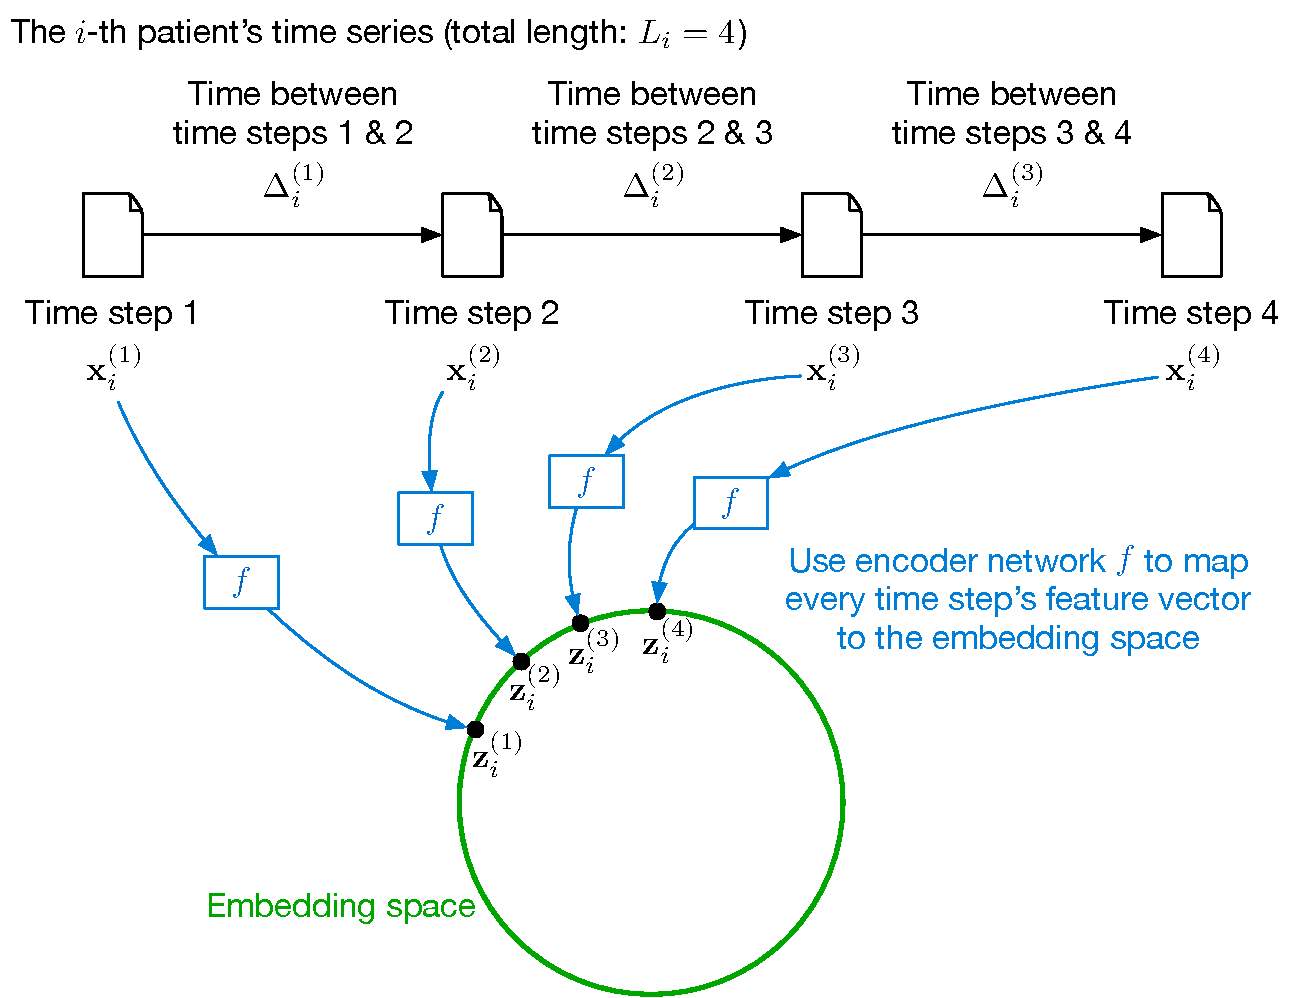
\includegraphics[width=0.48\linewidth,trim={6pt 0pt 6pt 6pt},clip]{Chapters/chapter-02/images/temporal-supervised-contrastive-learning-draft2-step1.pdf}
        } \\[.5em]
        \subfigure[Encourage temporal smoothness]{%
            \label{ch02:fig:temporal-smoothing}%
            \centering
            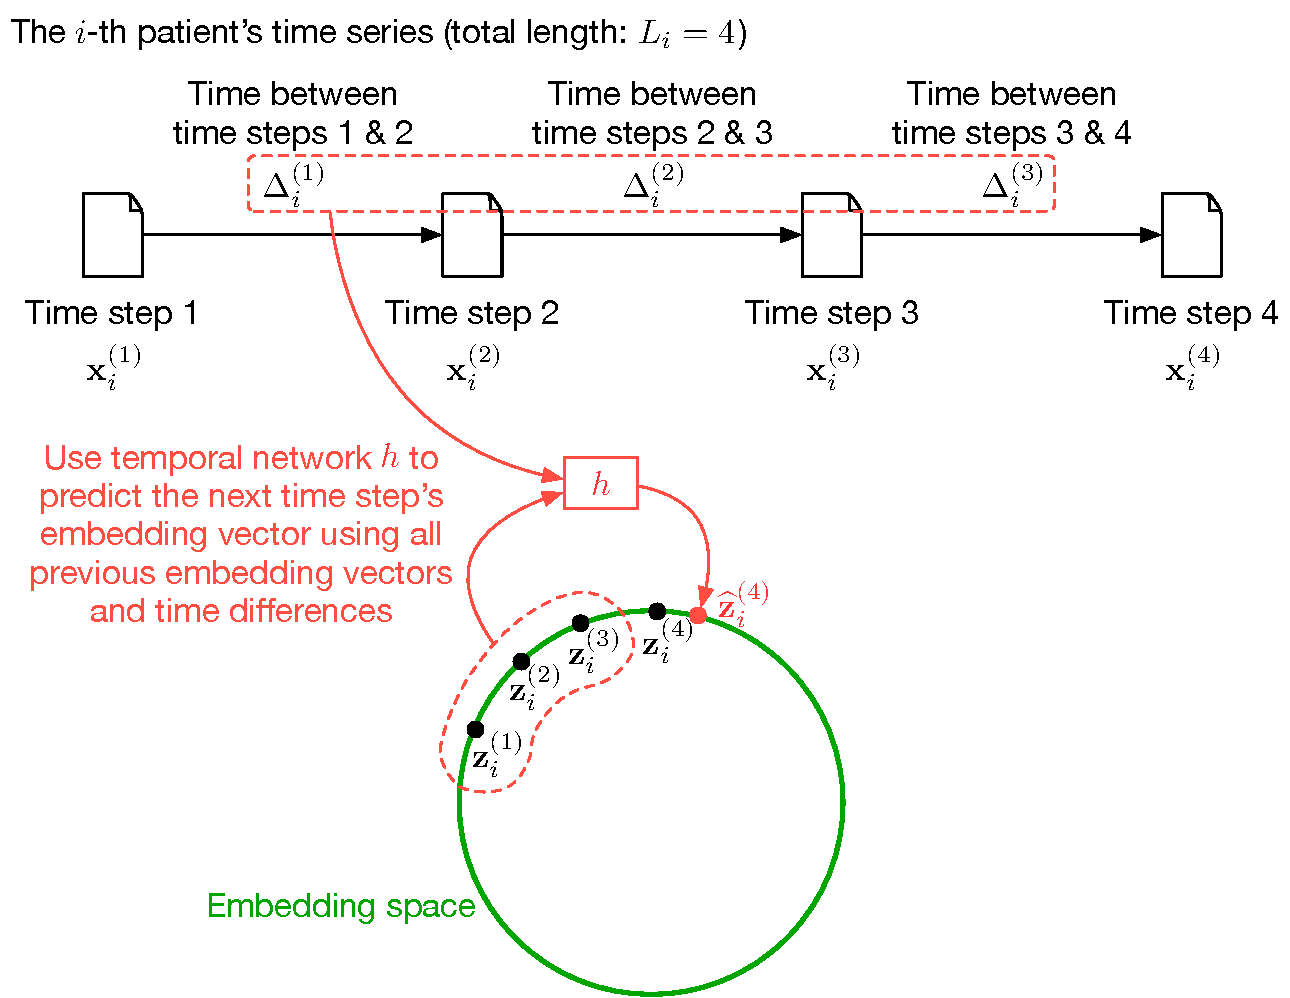
\includegraphics[width=0.48\linewidth,trim={6pt 0pt 6pt 6pt},clip]{Chapters/chapter-02/images/temporal-supervised-contrastive-learning-draft2-step2.pdf}
        } \\[0em]
        \subfigure[Predict using encoded representation]{%
            \label{ch02:fig:prediction}%
            \centering
            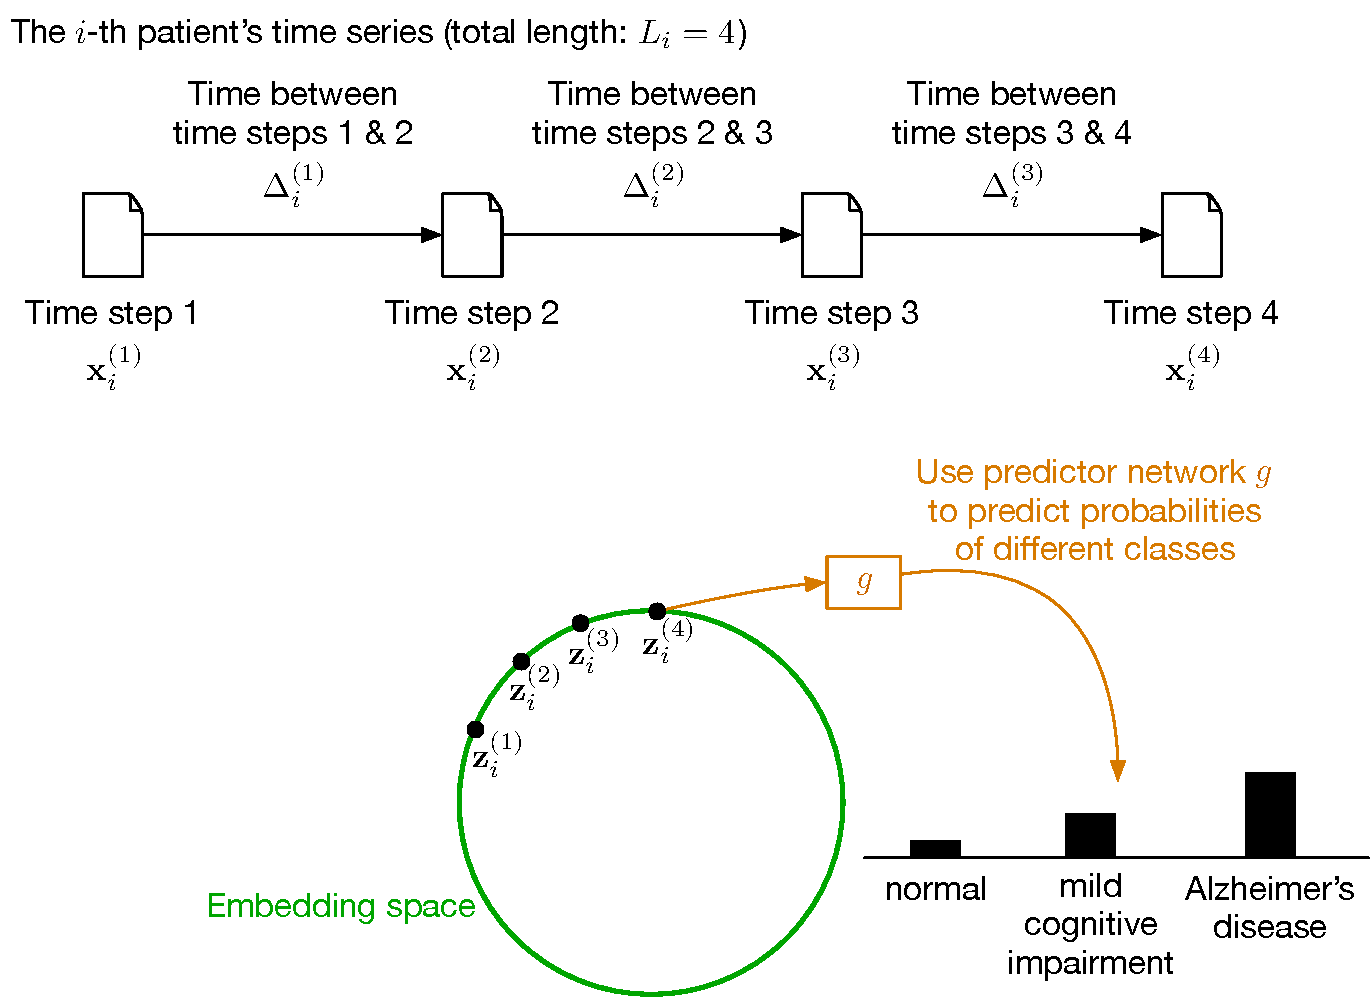
\includegraphics[width=0.48\linewidth,trim={6pt 0pt 6pt 21em},clip]{Chapters/chapter-02/images/temporal-supervised-contrastive-learning-draft2-step3-classification-version.pdf}
        }
        
    }
\end{figure}


\noindent
\textbf{Training.}
We train \ChTwoSmallCaps{Temporal-SCL} in three phases:
\begin{enumerate}

\item (Pre-training) We initialize the embedding space by pre-training the encoder~$f$ using data at the individual time step level and \mbox{\ChTwoSmallCaps{Simple-SCL}}. 
Note that during this phase, we do not model nor use temporal structure, and we effectively treat the different time steps as separate.
We explain this phase in more detail in Section~\ref{ch02:sec:learning-the-encoder}, and our experiments later show that this phase significantly improves the model's prediction accuracy.

\item (Encoder and temporal network training) After pre-training the encoder $f$, we account for temporal structure by jointly training $f$ and the temporal network $h$.
Details of this phase are in Section~\ref{ch02:sec:transform}.

\item (Learning the predictor network) At this point, we treat the encoder $f$ as fixed, so we can compute all the training embedding vectors at different time steps (the $\mathbf{z}_i^{(\ell)}$ variables).
In the dynamic outcome case, we learn the predictor network $g$ by treating the $\mathbf{z}_i^{(\ell)}$ variables as input feature vectors and the corresponding $y_i^{(\ell)}$ variables as target labels, minimizing cross-entropy loss.
In the static outcome case, we instead set the target label for $\mathbf{z}_i^{(\ell)}$ to be the final time step's label $y_i^{(L_i)}$.
As this phase amounts to standard neural net classifier training with cross-entropy loss, we omit further details.

\end{enumerate}
For ease of exposition, we explain the first two phases in Sections~\ref{ch02:sec:learning-the-encoder} and~\ref{ch02:sec:transform} only for the dynamic outcome case that we described in Section~\ref{ch02:sec:problem-setup}; the static outcome case is very similar and covered in Appendix~\ref{ch02:sec:handling-static-outcome}.


\noindent
\textbf{Prediction.}
At test time, we are given a feature vector $\mathbf{x}_*\in\mathbb{R}^{D}$ for a single time step.
To make a prediction for~$\mathbf{x}_*$, we first compute the embedding vector of $\mathbf{x}_*$ given by $\mathbf{z}_* \triangleq  f(\mathbf{x}_*)$.
Then the predicted class probabilities are precisely given by $g(\mathbf{z}_*)$.


\subsubsection{Pre-training the Encoder}
\label{ch02:sec:learning-the-encoder}


We now explain how we adapt \ChTwoSmallCaps{Simple-SCL} to time series data and to encourage learned embedding vectors to be diverse in capturing raw feature heterogeneity.
The latter uses a \emph{nearest neighbor pairing} mechanism.
We first pre-train our encoder network $f$ following a similar process as the \ChTwoSmallCaps{Simple-SCL} encoder, with specific modifications described below.


\noindent
\textbf{\ChTwoSmallCaps{Simple-SCL} encoder with time steps.}
Encoder of \ChTwoSmallCaps{Temporal-SCL}, $f$, has the same structure as \ChTwoSmallCaps{Simple-SCL} encoder.
We define every time step of every time series as its own \emph{snapshot}:  $(\mathbf{x}_i^{(\ell)}, y_i^{(\ell)})$.
Thus, we take the ``training data'' of our encoder network to be all the snapshots: $\bigcup_{i=1}^N \bigcup_{\ell=1}^{L_i} \{ (\mathbf{x}_i^{(\ell)}, y_i^{(\ell)}) \}$.


\noindent
\textbf{Nearest neighbor pairing for identifying similar snapshots.}
\label{ch02:sec:nearest-neighbor-refinement}
Whereas \ChTwoSmallCaps{Simple-SCL} (that did not have time steps) considered two points to be similar if they share the same classification outcome, we now instead consider two \emph{snapshots} to be similar if they share the same classification outcome \emph{and} their raw feature vectors are ``close to each other''.
We use random sampling to find pairs of similar snapshots:
\begin{enumerate}
\small
\item Initialize the set of snapshot pairs to be empty: $\mathcal{E} \leftarrow \emptyset$.
\item For each class $c\in[C]$:
\begin{enumerate}
\item 
Let the set $\mathcal{A}_c$ consist of all snapshots with label $c$.
\item While $|\mathcal{A}_c| \ge 2$:
\begin{enumerate}
\item Choose snapshot $(\mathbf{x}_i^{(\ell)}, y_i^{(\ell)})$ randomly from $\mathcal{A}_c$.
\item (Nearest neighbor search) Among the other snapshots in $\mathcal{A}_c$, find the one whose feature vector is closest to $\mathbf{x}_i^{(\ell)}$ (e.g., using Euclidean distance).
Denote the snapshot found as~$(\mathbf{x}_{i'}^{(\ell')}, y_{i'}^{(\ell')})$.
\item Add snapshot pair $\big((\mathbf{x}_i^{(\ell)}, y_i^{(\ell)}),(\mathbf{x}_{i'}^{(\ell')}, y_{i'}^{(\ell')})\big)$ to~$\mathcal{E}$.
\item Remove $(\mathbf{x}_i^{(\ell)}, y_i^{(\ell)})$ and $(\mathbf{x}_{i'}^{(\ell')}, y_{i'}^{(\ell')})$ from $\mathcal{A}_c$.
\end{enumerate}
\end{enumerate}
\end{enumerate}
To sample a minibatch of $B$ data points for minibatch gradient descent, where we assume that $B$ is even, we randomly choose $B/2$ pairs from the set $\mathcal{E}$; denote the set of these $B/2$ pairs as $\mathcal{E}_{\text{batch}}$.
Note that the $B/2$ pairs in $\mathcal{E}_{\text{batch}}$ correspond to a total of $B$ different snapshots; denote the set of these $B$ snapshots as $\mathcal{V}_{\text{batch}}$.
Then the loss we use for minibatch gradient descent during pre-training is
\begin{align*}
    &L_{\text{SCL-snapshots}} \triangleq \\
    &- \!\!\!\!\!\!\!\!%
    \sum_{\substack{((\mathbf{x}_i^{(\ell)}, y_i^{(\ell)}), \\ ~\!(\mathbf{x}_{i'}^{(\ell')}, y_{i'}^{(\ell')})) \\ ~\!\in~\!  \mathcal{E}_{\text{batch}}}} \!\!\!\!\!\!%
    \log\Bigg[
\frac{\exp(\langle f(\mathbf{x}_i^{(\ell)}), f(\mathbf{x}_{i'}^{(\ell')}) \rangle / \tau)}{\sum\limits_{\substack{(\mathbf{x}_{i''}^{(\ell'')}, y_{i''}^{(\ell'')}) ~\!\in~\!  \mathcal{V}_{\text{batch}} \\ \text{~s.t.~}(i'',\ell'')\ne(i,\ell)}} \!\!\!\!\!\!\!\!\!\!\!\!\!\!\!\exp(\langle f(\mathbf{x}_i^{(\ell)}), f(\mathbf{x}_{i''}^{(\ell'')}) \rangle / \tau)}\Bigg]
\end{align*}
For simplicity, our experiments later use Euclidean distance to find nearest neighbors (we standardize features to control for scale differences), efficiently computed using fast approximate nearest neighbor search software \citep{malkov2018efficient}.


% !TeX root = ../../../main.tex
\begin{figure}[t!]

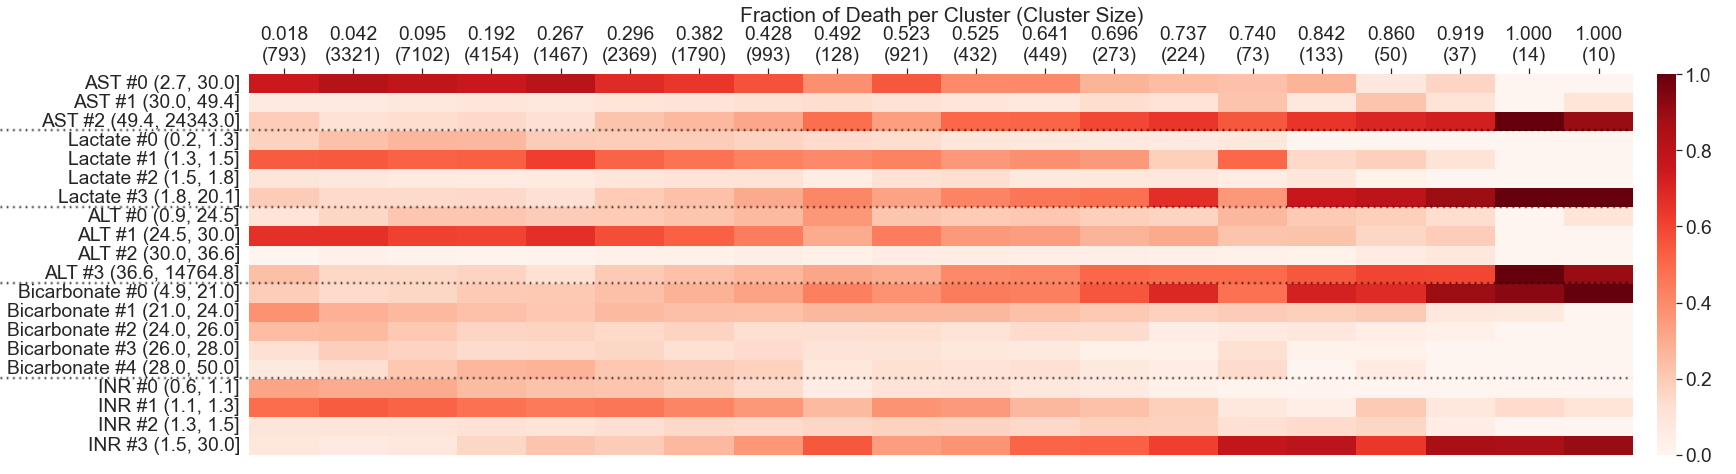
\includegraphics[width=1\linewidth]{Chapters/chapter-02/images/mimicHeatmap.png}

 \caption{Heatmap showing how features (rows) vary across clusters (columns) for the sepsis cohort of the MIMIC dataset. Heatmap intensity values can be thought of as the conditional probability of seeing a feature value (row) conditioned on being in a cluster (column); these probabilities are estimated using test set snapshots. Columns are ordered left to right in increasing fraction of test set snapshots that come from a time series that has a final outcome of death.
 }   \ChTwoFloatLabel{ch02:fig:heatmapMIMIC}
\end{figure}


\noindent
\textbf{Ablation.}
Later on in our experiments, we conduct ablation experiments where we do not use nearest neighbor pairing.
The only change is that in step 2(b), steps i.~and ii.~are replaced by randomly choosing two different snapshots $(\mathbf{x}_{i}^{(\ell)}, y_{i}^{(\ell)})$ and $(\mathbf{x}_{i'}^{(\ell')}, y_{i'}^{(\ell')})$ from $\mathcal{A}_c$ to pair up (uniformly at random).



\noindent
\textbf{Note on data augmentation.}
A key component of contrastive learning is \emph{data augmentation} (see the review by \citet{le2020contrastive}), a procedure that creates perturbed versions of data points (e.g., when working with images, we could randomly rotate, translate, and crop an image).
Since we work with tabular data, a challenge arises in that to the best of our knowledge, there is no widely accepted, clinically suitable data augmentation method for such data.
Thus, our presentation of \ChTwoSmallCaps{Temporal-SCL} is \emph{without data augmentation}; in fact, the nearest neighbor pairing mechanism proposed above is also a substitute for data augmentation. %TODO: Add why
While we do not use data augmentation, we point out that if it is available, adding it is trivial.
The simplest way is that before each training epoch, we apply data augmentation to the original training dataset to get a fresh augmented training dataset, which we use with our nearest neighbor pairing procedure.
More details are in Appendix~\ref{ch02:sec:data-augmentation-with-nn-pairing}.



\subsubsection{Encoder and Temporal Network Training}
\label{ch02:sec:joint-optimization}

 
\label{ch02:sec:transform}

In the second stage of training a \ChTwoSmallCaps{Temporal-SCL} model, we jointly train the encoder and temporal networks by minimizing the overall loss
\begin{align}
    L_{\text{overall}} &=L_{\text{SCL-snapshots}}+ \alpha L_{\text{temp-reg}},
\label{ch02:eq:mainLoss}
\end{align}
where $L_{\text{temp-reg}}$ is a temporal smoothness loss term (to be defined shortly), and ${\alpha\ge0}$ is a hyperparameter that trades off between the two losses on the right-hand side.
Recall that for the \mbox{$i$-th} training data point, we previously defined the time duration $\delta_i^{(\ell)}\triangleq t_i^{(\ell+1)} - t_i^{(\ell)}$ for $\ell=1,2,\dots,{L_i-1}$. 
Moreover, $h$ takes as input the sequence $\{(\mathbf{z}_i^{(t)},\delta_i^{(t)})\}_{t=1}^{\ell}$ and outputs a prediction for $\mathbf{z}_i^{(\ell+1)}$. 
We ask that $\mathbf{z}_i^{(\ell+1)}$ and $h\big(\{(\mathbf{z}_i^{(t)},\delta_i^{(t)})\}_{t=1}^{\ell}\big)$ be close by squared Euclidean distance, across all data points and time steps:
\begin{align*}
&L_{\text{temp-reg}}
\!\triangleq \!\!\!\!\!
&\!\frac{1}{N}\!\sum_{i=1}^N  \! \sum_{\ell=1}^{L_i - 1} \! \frac{
\big\| h\big(\{(\mathbf{z}_i^{(t)},\delta_i^{(t)})\}_{t=1}^{\ell}\big)
\!-\! \mathbf{z}_i^{(\ell+1)} \big\|^2 }{L_i-1}.
\end{align*}


\subsubsection{Visualizing Embedding Vectors}
\label{ch02:sec:visualizing}


To find common patterns in the learned embedding space, we cluster on the different snapshots' embedding vectors (the $\mathbf{z}_i^{(\ell)}$ variables) \emph{after} training a \ChTwoSmallCaps{Temporal-SCL} model.
We have found standard agglomerative clustering \citep{murtagh2012algorithms} to work well here and this approach trivially allows the user to adjust the granularity of clusters as needed, even from fitting the clustering model once.
The idea is that we start with every snapshot's embedding vector as its own cluster and keep merging the closest two clusters (e.g., using complete linkage to decide on which two clusters are closest) until we are left with a single cluster that contains all the snapshots' embedding vectors.
In conducting this procedure, we store each intermediate clustering result.
Then the user could use our visualization strategy (to be described next) with any intermediate clustering result, ranging from fine- to coarse-grain clusters.

To visualize \emph{any} cluster assignment of the snapshot embedding vectors (the clustering method need not be agglomerative clustering), we make a heatmap inspired by \citet{li2020neural}, where columns correspond to different clusters and rows correspond to features.\footnote{Note that we discretize continuous features into bins. This discretization is only used during visualization and not used when training the \mbox{\ChTwoSmallCaps{Temporal-SCL}} model.} The intensity value at the $i$-th row and $j$-th column is the fraction of test set snapshots that have the $i$-th row's feature value among test set snapshots in the $j$-th column's cluster (i.e., a conditional probability of seeing a feature value given being in a cluster).
An example is shown in Fig.~\ref{ch02:fig:heatmapMIMIC}; details on the dataset used and model training are in Section~\ref{ch02:sec:ClinicalExperiments}. 
We show the ``top'' 5 features,
where we rank features based on the maximum observed difference across clusters.\footnote{Per row in the heatmap, compute the difference between the largest and smallest intensity values across the row, and rank rows using these differences, where we keep rows that correspond to the same underlying feature together.}


